\chapter{Thesis model code \label{apx:modelcodeoverview}}

\section{Introduction}

This appendix describes the models produced specifically for the thesis. A download link to a single `zip' file containing these can be found via:

\begin{itemize}
\item \textbf{http://bit.ly/olnerthesis2013}
\end{itemize}

This zip file contains the following:

\begin{itemize}
	\item ``CoreModel'' folder: contains a runnable jar file for the core model version in section \ref{sec:coremodel}. Instructions are included in a ``readme.txt'' file in the folder.
\item ``FrameWorkModelBuilds'' folder: contains a series of runnable jar files for the thesis models. ``listOfModels.txt'' explains them and links to the sections of the thesis they appear in. 
\item ``EoS\_vs\_LoV\_ExcelModel\_DanOlner2013web.xlsx'': the spreadsheet version of the `transmission belt' mechanism section from section \ref{sec:transmissionbelttrackinz}.
\item ``exchangetestrandom'': Matlab file for the random money exchange example, section \ref{sec:comm_costs}.
\end{itemize}

`Jar' files need to stay in their folders to run as they rely on the libraries and config files there. They should be openable by double-clicking. If this does not work, the command line can be used. Navigate to the `scenarios' folder, and use:

\begin{quote}
java -jar ``*filename*.jar''
\end{quote}

Section \ref{sec:uml} explains the UML overview diagram given at the end of the appendix, and goes into more detail on the structure of those classes and their role in the model framework.
%The CD included with the thesis has the Javadoc, which can be opened in a browser, and contains all classes. To open the Javadoc, navigate into the `Javadoc' folder and open `index.html' (double-clicking should open in the default browser). The CD also includes the source code in the `Location1' folder. 

Section \ref{sec:modelsCD} describes the runnable models included in the ``FrameWorkModelBuilds" folder and explains the interactive features available in those that were used as a virtual laboratory in the thesis. 

A quick final note on the use of floating point numbers: for the vast majority of modelling problems covered in this thesis, the choice of floating point numbers presented no problem, despite their well-documented issues (see e.g. \citealt{polhill_what_2006}). However, those floating points issues do exist, particularly where many interdependent Actors attempt to equilibriate some value to zero. A way to fix this would be to use very large integer values, but this would require a ground-up recoding. 

\section{UML overview \label{sec:uml}}

Figure \ref{fig:UML}, at the end of the appendix, provides a UML overview of the model classes. It does not include all classes (see the Javadoc for these) but provides an overview of all the main and abstract classes, such as `Actor', that have more than one extension. The following list briefly explains each class in the UML overview. 
%Elements of figure \ref{fig:UML} are numbered. Those numbers correspond to the following description.

\begin{enumerate}
	\item Main: runs through the top-level model setup, including:
\begin{itemize}
	\item use gl.setUp() to set global variables, number of agents etc.
	\item	Parameter-sweep loops, call each modelRun() and changes values
	\item modelRun(): set up each individual run, includes:
	\begin{itemize}
		\item ActorMaker.makeActors
		\item set up visualisations
		\item set initial actor locations
		\item set up Action permuters
		\item set up data `Buckets'
		\item iterate through single run day number
	\end{itemize}
	\end{itemize}%end main subitems
	\item TimeLine: the main `audible' class (see below) that many others use as a reference to know when to act. TimeLine's day is iterated in modelRun().
	\item `gl': short for Global, shortened version used for quick reference to global variables. `gl' sets up all of these global variables; other classes use it extensively both for storing and retreiving global variables.
	\item ActorMaker: instantiates all Actors, goes their action setup and does any specific jobs like setting variable spreads across Actors.
	\item Space: contains all methods related to geography, including methods for Actors to get a list of `whosInRadius' relative to their location, or the location of a Bundle they are testing. Also does the following: finds density cost; provides methods for setting Actor location in desired patterns; deals with wrapping if model is a torus or `racetrack' (wrapping line); implements Drawable, so takes care of carrying out drawing of geographical visualisations
	\item Actor: top-level object over-written by sub-types Person, Firm, SingleActorPerson
	\item Action: again, overwritten for particular actors by PersonAction, FirmAct and SingleActorAction
	\item UtilityShell and ProductionShell: wrappers, each wrapping a `giveUtility' or `giveOutput' method for a swappable Utility or Production class. 
	\item Bundle: a collection of Goods and their sellers and locations, each of which gets its own utility level when maximised.
	\item Good: single good, containing details of cost, seller and temporary values when maximising. A Good can be sold by any class implementing the `GoodSeller' interface, so People can – in the single Actor models – sell as well as buy.
	\item ProcessingDrawer: puts an inner class Processing applet into a frame and has an array of Drawables who are asked to draw when `heard'. 
	\item Important interfaces (see below for others in the `observe' classes).
		\begin{itemize}
			\item HasLocation: guarantees that Space's methods can work on any class implementing
			\item Drawable: any class that implements this and registers with a Drawer will have the Processing applet passed to its `draw' method when `heard'. It is then up to the class how and what it draws, within the framework of a particular Drawer. 
		\end{itemize}
	\item Output classes:
		\begin{itemize}
			\item DataStore: holds all the `Buckets', implements listener, calls Buckets to get data when `heard'. Can be used to store single or multi-run data.
			\item Bucket: extended by particular `Buckets' that will deal with storing the required data.
			\item CSVWriter: two versions of this – one listens for the end of model runs to write data, the other is static and will write data at any required point.
		\end{itemize}
	\item `Observer' classes
		\begin{itemize}
			\item Audible (interface): any class that wants to be audible to Listeners. In theory could be used for event-driven model, but in practice, only TimeLine currently implements Audible.
			\item Listener (interface): any class that wants to know about what day it is needs to implement this and provide a Shouter to an Audible.
			\item Shouter: keeps a record of its Listener, lets it know when its been asked to shout. 
			\item ListenerWrapper: wraps Listener's `heard' method, so that Listeners can be exchanged at runtime. Used by the visualisation mouse control system. 
		\end{itemize}	
\end{enumerate}

\section{Framework outline \label{sec:modelsCD}}
\subsection{Visualisation and interaction}

%%%%%%%%%%%%%%%%%%%%%
\subsubsection{Main visualisation window}

The main visualisation window will display the visualisations as described in the relevant sections of the results chapter. Each scenario is listed below, with a reference to the appropriate section. The window also provides menus for changing the assignment of variables to mouse buttons. These are top-left, just called `mouse1' and `mouse2'. When selected, clicking and dragging with the left (mouse1) or right (mouse2) vertically will change values. The current value is displayed bottom left. The variables are repeated in each menu. Those available vary from model to model, but will include the following:

\begin{itemize}
	\item deliv: sets good delivery cost for all goods
	\item wage: sets all Firms' wage offer
	\item price: sets all Firms' good base price
	\item tech: If People have to `pay' distance to work, this sets the `tech' element
	\item CES: If a CES utility function is used, this sets $\rho$.
	\item model: Controls model view angle by dragging
	\item density: sets density cost level for all People
	\item uViz: changes magnitude of visualisation of utility levels
	\item lViz: changes magnitude of visualisation of buying levels
\end{itemize}

There are also a number of toggle buttons. Some are specific to particular scenarios, but the common ones are:

\begin{itemize}
	\item peoplemove: toggle whether People are able to change location
	\item firmsmove: toggle whether Firms are able to change location
	\item wageTime: toggle whether People must `pay' the commute time to Firms
\end{itemize}

%%%%%%%%%%%%%%%%%%%%%
\subsubsection{Graph visualisation}

For those models that include a graph output, note the following:

\begin{itemize}
	\item Graphs default to showing a moving record of 400 values. `f' will turn on or off the following behaviour.
	\item The graph will find the lowest and highest value and display between them. It will fix to the highest, so if values drop, the graph can be reset by pressing `r'. 
\end{itemize}

All scenarios can be exited by pressing escape while the focus is on the main visualisation window. 

\subsection{List of scenarios}

As mentioned, the `ModelBuilds' folder contains a description of each included scenario and the section it relates to – this is included here for quick reference:

\begin{itemize}

\item MonoCentricDensity (section 5.4.7: ``Spatial equilibria are not always utility equilibria''): Starts with density cost = 100, at the point where two bands of utility indifference emerge. Two correlation graphs show density and utility versus distance from centre. 

\item TwoFirmsLineMove2000dayAverage (section 5.5.1: ``Two Firms optimising location on a line''): Two firms on a 1d line of length one compete for demand by moving location only. Fifty People spread evenly along the line from $0$ to $1$. Means taken over $2000$ timesteps for Firm position and People's demand. White arrows shows Firms' mean location; white bars show one standard deviation each side of this; thin black vertical lines show actual positions taken by Firm over previous $2000$ timesteps. Timestep value to average over can be changed via the config file ``Hotelling\_Line\_DMR.properties'' in the `configs' folder.

\item `SymmetryBreak' (section 6.4: ``Introducing space into the transmission model'') folder contains the following two jars:

\begin{itemize}

\item SymmetryBreakParameterSweep: Greyed out correlation graph will fill with datapoints as the model sweeps up rho and delivery costs in turn. Main visualisation window blocks: Firms' time input from People.

\item SymmetryBreakParameterSweepFast: after 500 days, model run speeds up to show full range of transitions quickly and the way each Firm reacts. Main visualisation window blocks: Firms' time input from People.

\end{itemize}

\item ManyAgentsLineTransmissionBelt (section 6.4.1: ``Space and welfare outcomes in a many-agent model''): line of 19 firms/people set at point that transition to a single more-efficient producer will emerge. Mouse is linked to rho (left button) and distance costs (right button). Increase distance costs to return the model to the spread equilibrium. Increasing rho (increasing substitutability of goods) will in turn allow efficient production to re-emerge. At higher distance costs, more than one efficient producer will emerge.

\item TransmissionBeltPlusDensity (section 6.4.2: ``Combining the transmission belt model with density cost''): Two firms a distance of 1 apart, 300 people. If rho is raised (left-mouse click and drag up) at  ~rho=0.9, transition to single more-efficient producer takes place, People move, create settlement there, buy in from further firm.

\item TwoRegionFourFirmsTransmissionBelt (section 6.4: ``introducing space into the transmission belt model''): discrete two region model with two Firms per region. For values of rho and distance cost (attached to mousebutton 1 and 2) four different production regime types emerge (see section 6.4).

\end{itemize}

\begin{sidewaysfigure}
\centering
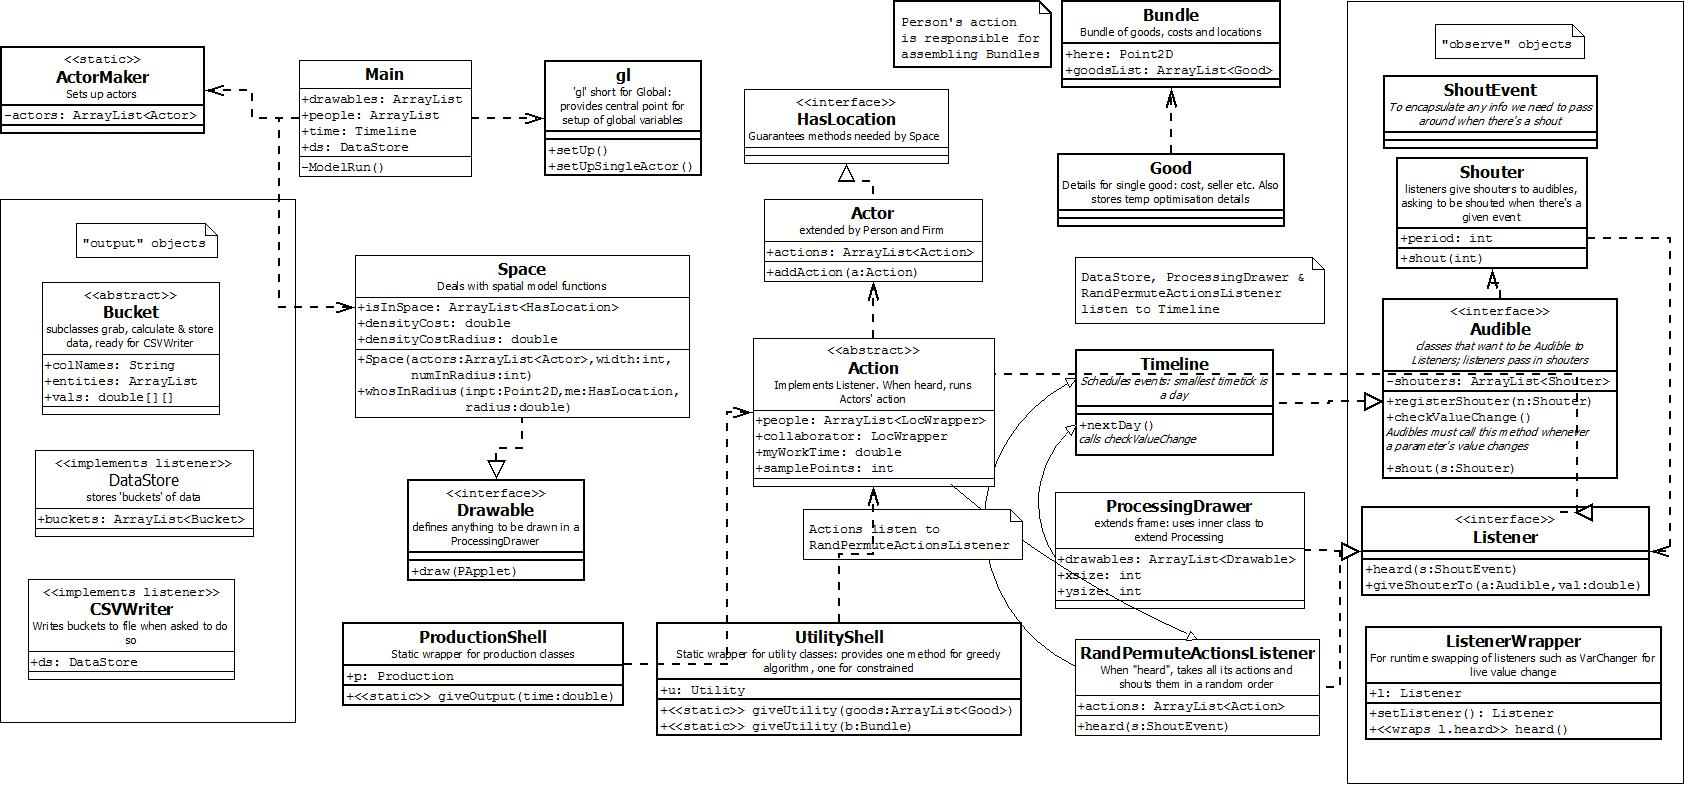
\includegraphics[width=1\columnwidth]{Appendices/location1_UML}%
\caption{Model framework UML overview \label{fig:UML}}%
\end{sidewaysfigure}
